\documentclass{recipe}

\begin{document}
\begin{recipe}{Thai Red Curry}
  \servings{3}

  \begin{ingredients}
    \ingredient{3}{}{chicken thighs}
    \ingredient{1}{tbsp}{butter}
    \ingredientsep
    \ingredient{8}{oz}{coconut milk}
    \ingredient{1}{tbsp}{thai curry powder}
    \ingredient{2}{cloves}{garlic}
    \ingredient{}{}{basil}
    \ingredient{}{}{cayenne pepper}
    \ingredient{}{}{paprika}
    \ingredient{}{}{salt}
    \ingredientsep
    \ingredient{1}{cup}{rice}
  \end{ingredients}

  \begin{images}
    \begin{image}
      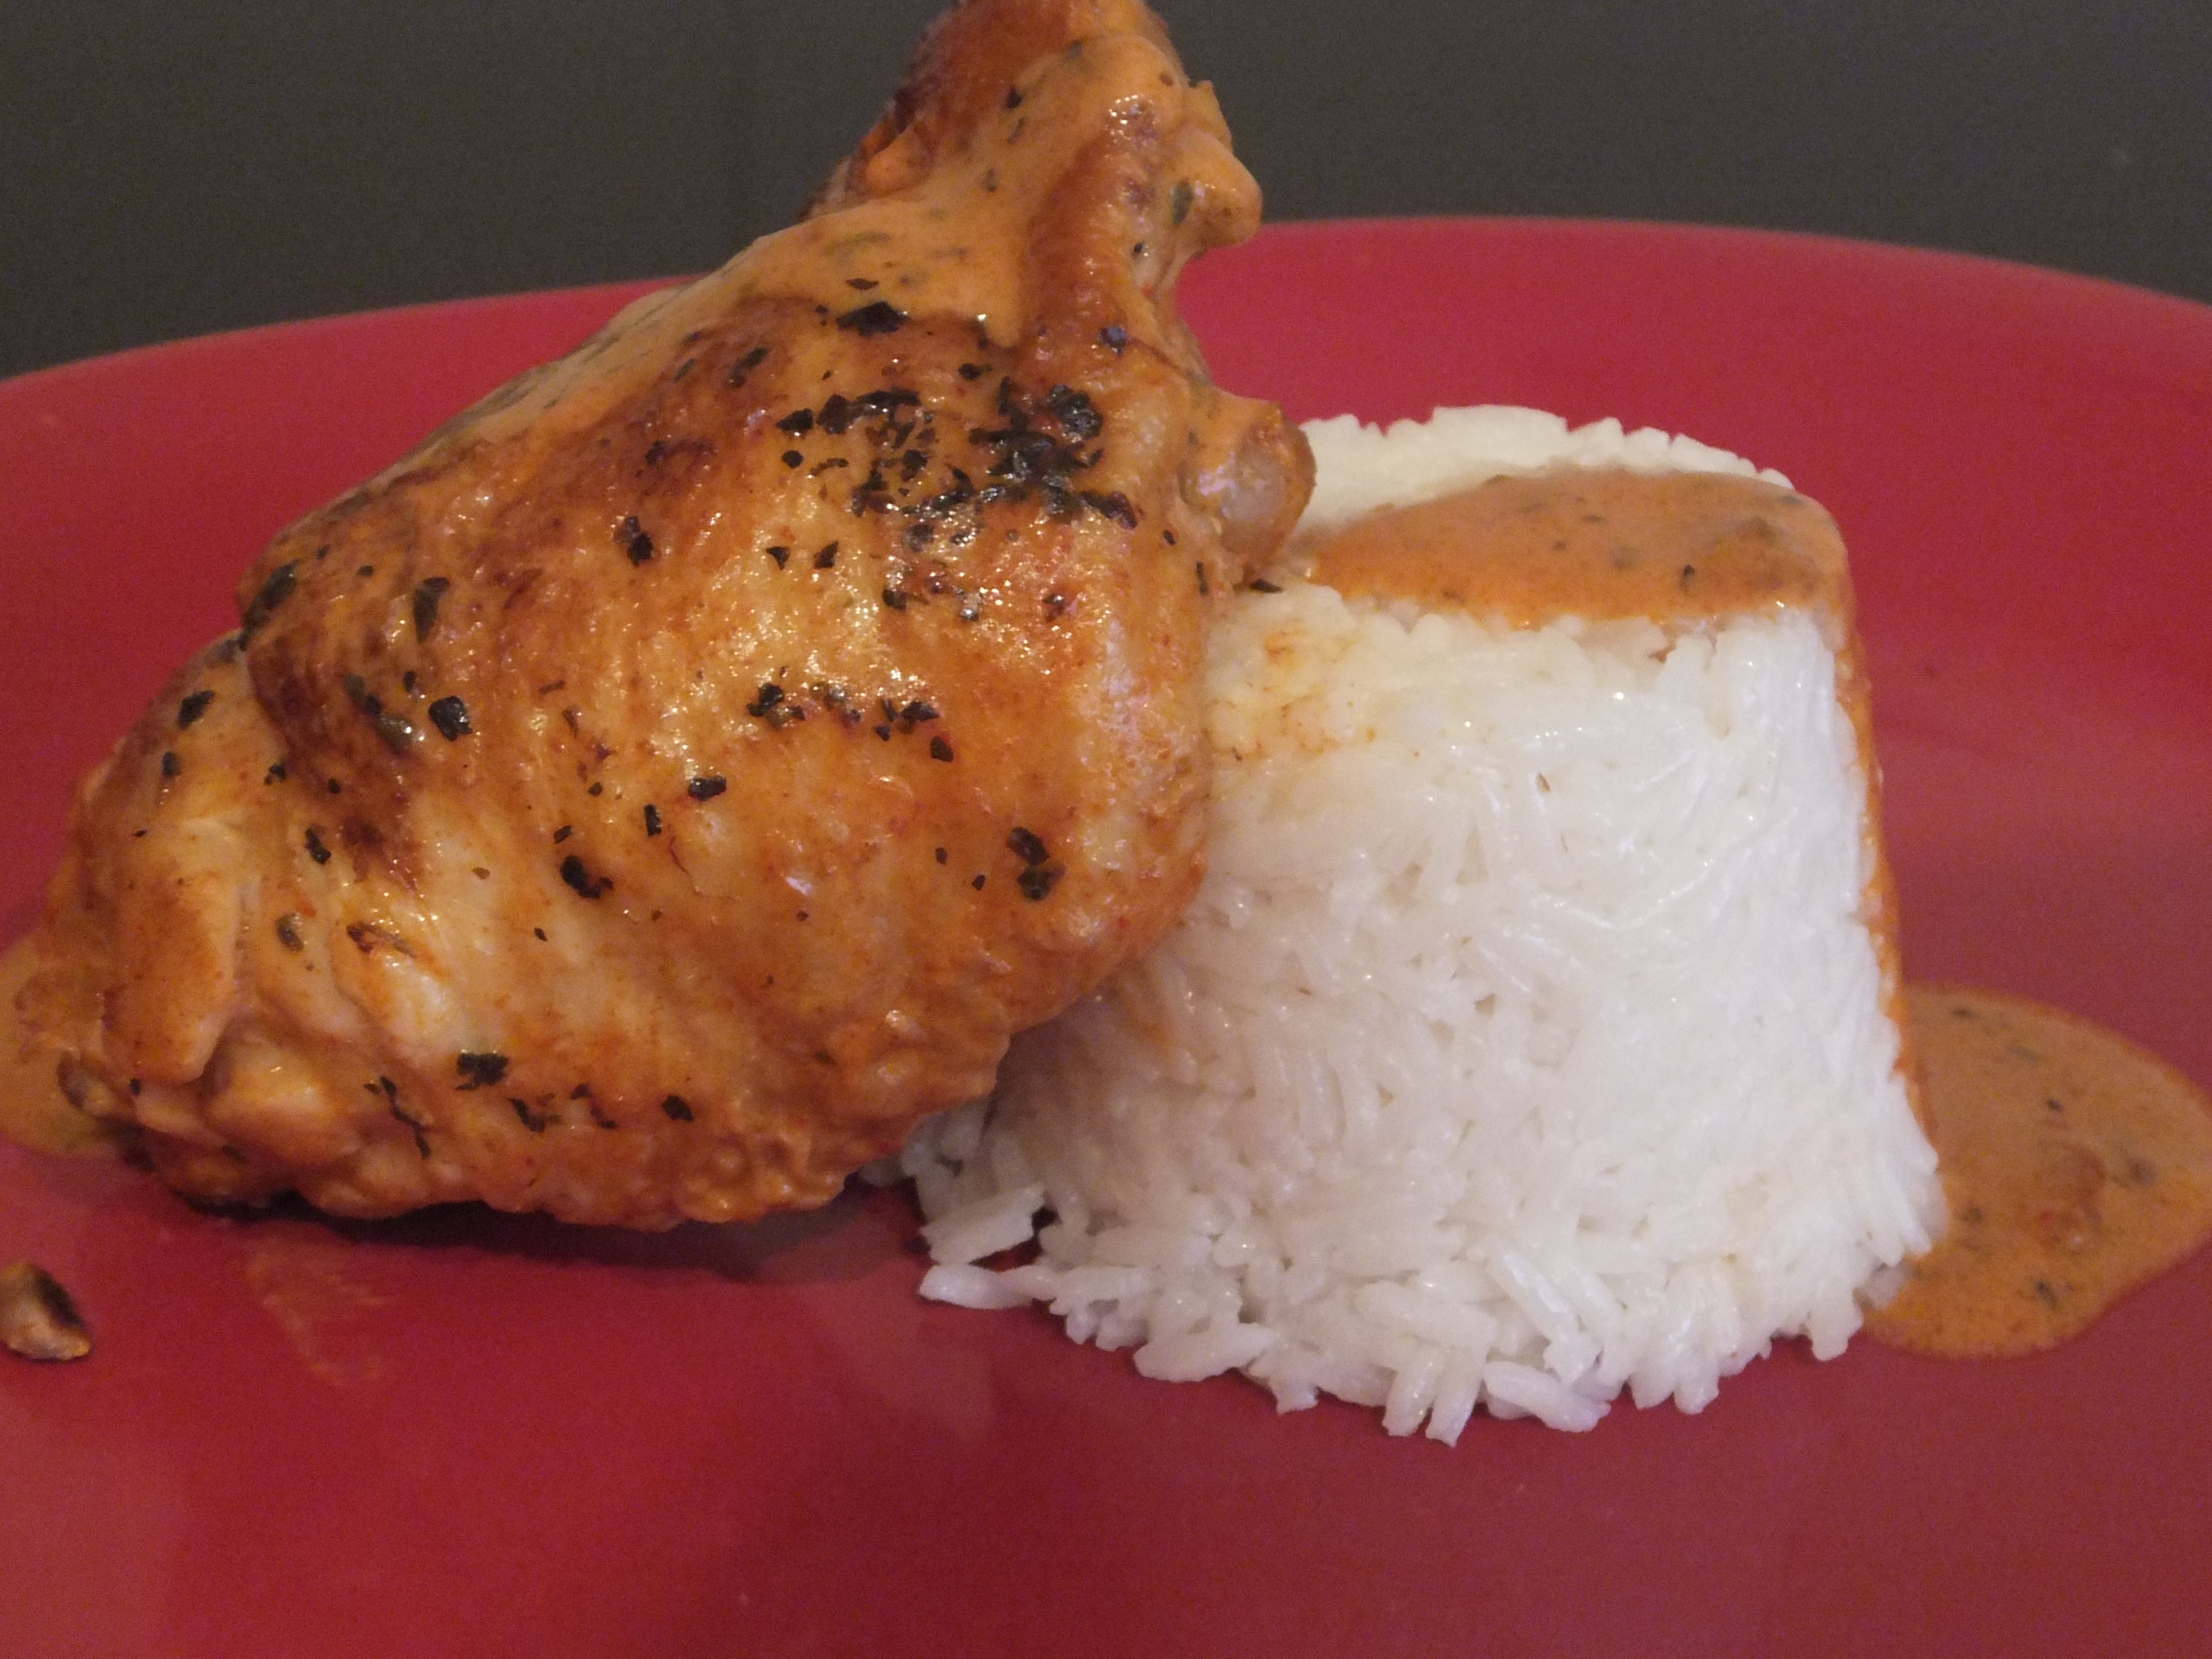
\includegraphics[width=\linewidth,trim=0px 0px 0px 0px, clip=true]{red_thai_curry-01.jpeg}
    \end{image}
  \end{images}

  \begin{steps}
  \item Set a pan on medium-high and put the chicken skin-side down into the
    butter.
  \item Render the chicken skin.
  \item Add some water, the coconut milk, and the spices to the pan and braise
    until the chicken is tender (45 minutes).
  \item Cok the sauce on low for a few minutes while the chicken rests
    and the rice finishes cooking.
  \item Serve with the rice.
  \end{steps}
\end{recipe}
\end{document}
